\documentclass[aps,pra,notitlepage,amsmath,amssymb,letterpaper,12pt]{revtex4-1}
\usepackage{amsthm}
\usepackage{graphicx}
%  Above uses the Americal Physical Society template for Physical Review A
%  as a reasonable and fully-featured default template
 
%  Below define helpful commands to set up problem environments easily
\newenvironment{problem}[2][Problem]{\begin{trivlist}
\item[\hskip \labelsep {\bfseries #1}\hskip \labelsep {\bfseries #2.}]}{\end{trivlist}}
\newenvironment{solution}{\begin{proof}[Solution]}{\end{proof}}
 
% --------------------------------------------------------------
%                   Document Begins Here
% --------------------------------------------------------------

% In what follows, you can easily change text to see what happens to the document
% For example, replacing the text "Document X" inside the "\title{}" command will
% change the document title
 
\begin{document}
 
\title{Parabolic Potential}
\author{Alley Busick}
\affiliation{PHYS 220, Schmid College of Science and Technology, Chapman University}
\date{\today}

\maketitle

\section{Parabolic Potential} % Specify main sections this way

% x.yz is the problem number
\begin{problem}{x.yz} 
Consider a ball of mass $m$ with horizontal coordinate $x$ rolling in a double-well potential $V(x) = x^4/4 - x^2/2$. Note that according to Newton's second law, the ball must satisfy the equation of motion: $$m\ddot{x} = f_{\text{hat}}(x) + f_{\text{drag}}(\dot{x}) + f_{\text{drive}}(t) = x - x^3 - \nu \dot{x} + F\cos(\omega t)$$ Your task will be to solve these equations numerically, for $m=1$, $\nu = 0.25$, and $\omega = 1$. Use a time-step size of $\Delta t = 0.001$ with the 4th-order Runge-Kutta integration method to keep sufficient numerical precision.
\end{problem}
 
\begin{solution} %You can also use proof in place of solution
Solved numerically, the 4th-order Runge-Kutta method was implemented to solve above equations with various $F$, $N$, $x_0$, and $y_0$ values (observation purposes). A derivative function was first used then the ODE function (following two graphing functions for the notebook).
% Use align environments for equations. The \\ is a newline character. The & is the alignment character.
% Using align* or \nonumber on each line removes equation numbers
\end{solution}

\subsection{Plotted Sombrero} % Specify subsections and subsubsections this way

Figures can be included easily.

\begin{figure}[h!] % h forces the figure to be placed here, in the text
  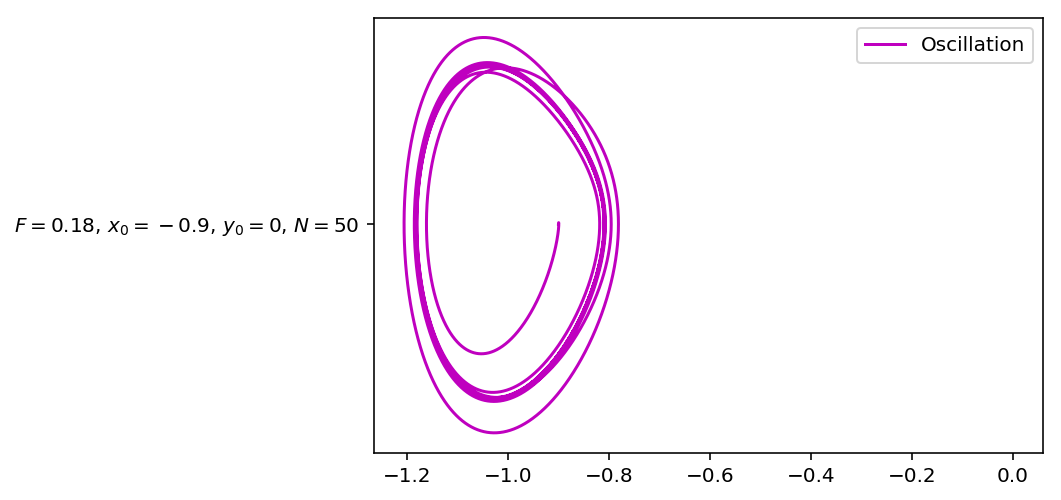
\includegraphics[width=0.4\textwidth]{-0.9.png}  % if pdflatex is used, jpg, pdf, and png are permitted
  \caption{Oscillation $x_0=-0.9$}
  \label{fig:figlabel}
\end{figure}

\begin{figure}[h!] % h forces the figure to be placed here, in the text
  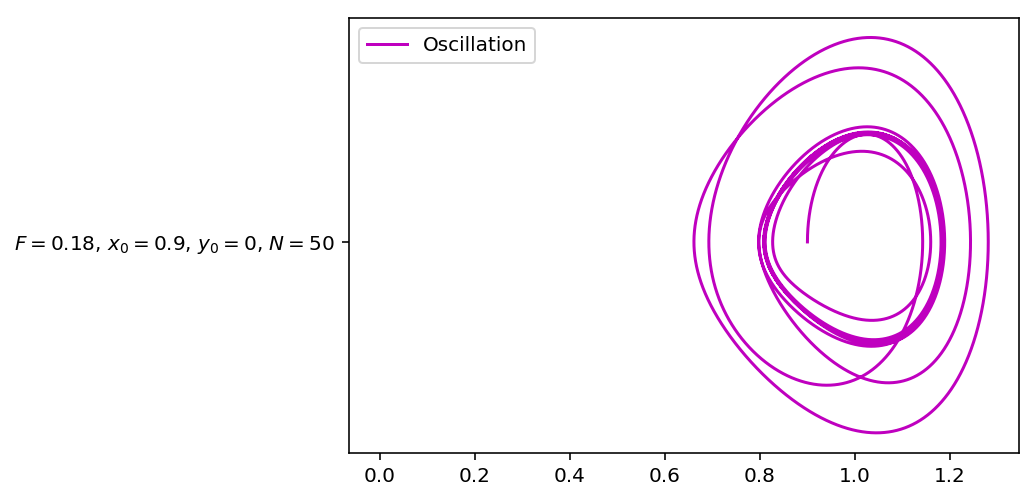
\includegraphics[width=0.4\textwidth]{0.9.png}  % if pdflatex is used, jpg, pdf, and png are permitted
  \caption{Oscillation $x_0=0.9$}
  \label{fig:figlabel}
\end{figure}

\begin{figure}[h!] % h forces the figure to be placed here, in the text
  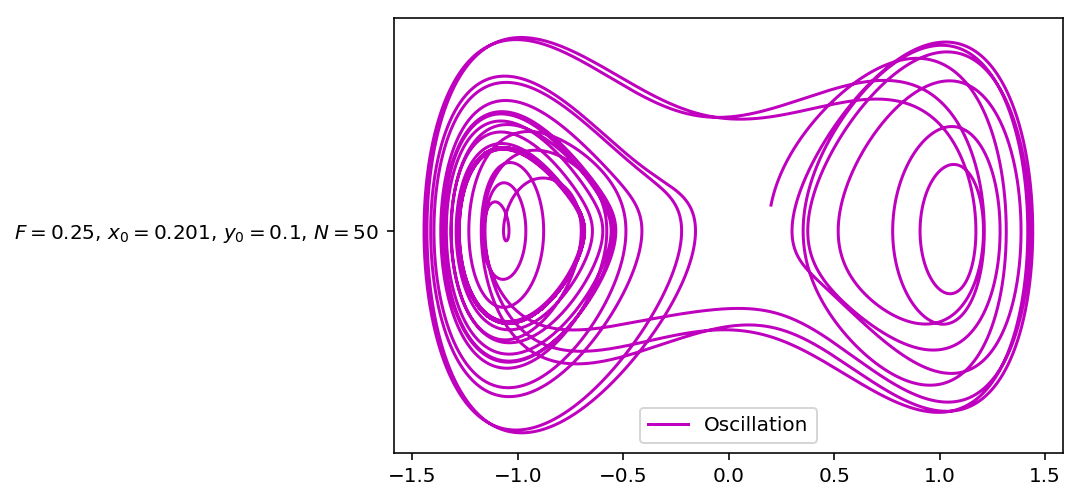
\includegraphics[width=0.4\textwidth]{0.201.png}  % if pdflatex is used, jpg, pdf, and png are permitted
  \caption{Oscillation $x_0=0.201$}
  \label{fig:figlabel}
\end{figure}

This text should be below the figure unless \LaTeX  decides that a different layout works better.
 
% Repeat as needed
 
\end{document}
